% Shared standalone design for the editable figure reconstructions.
\documentclass[tikz,border=5pt,10pt]{standalone}
\usepackage[T1]{fontenc}
\usepackage[utf8]{inputenc}
\usepackage{newpxtext,newpxmath}
\usepackage[scaled=.94]{sourcesanspro}
\usepackage{pgfplots}
\pgfplotsset{compat=1.18}
\usetikzlibrary{arrows.meta,calc,positioning,decorations.pathreplacing,
  decorations.markings,patterns,matrix,shapes.geometric,fit,backgrounds,
  intersections,angles,quotes}
\definecolor{ink}{HTML}{203746}
\definecolor{accent}{HTML}{146C78}
\definecolor{muted}{HTML}{667780}
\definecolor{signalred}{HTML}{B94B44}
\color{ink}
\tikzset{>=Latex,line width=.8pt,
  every node/.style={font=\small},
  axis/.style={->,draw=muted,line width=.5pt},
  guide/.style={draw=muted,dashed,line width=.45pt},
  curve/.style={draw=accent,line width=1pt},
  marker/.style={circle,fill=accent,inner sep=1.5pt},
  labelbox/.style={fill=white,inner sep=2pt}}

\begin{document}
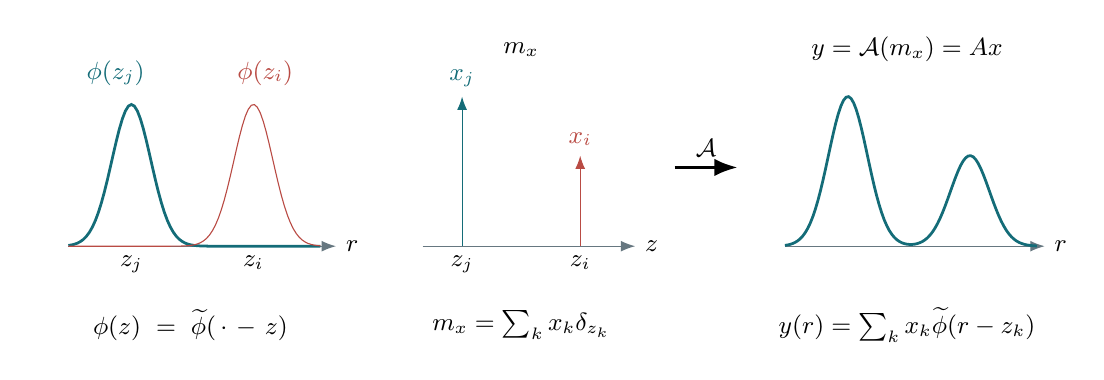
\begin{tikzpicture}
\begin{scope}
\draw[axis](0,0)--(3.4,0)node[right]{$r$};
\draw[curve]plot[domain=0:3.2,samples=85](\x,{1.8*exp(-((\x-.8)/.35)^2)});
\draw[signalred]plot[domain=0:3.2,samples=85](\x,{1.8*exp(-((\x-2.35)/.35)^2)});
\node[accent]at(.6,2.2){$\phi(z_j)$};\node[signalred]at(2.5,2.2){$\phi(z_i)$};
\node[below]at(.8,0){$z_j$};\node[below]at(2.35,0){$z_i$};
\node[align=center,text width=3.9cm]at(1.55,-1.0){$\phi(z)=\widetilde\phi(\,\cdot-z)$};
\end{scope}
\begin{scope}[shift={(4.5,0)}]
\draw[axis](0,0)--(2.7,0)node[right]{$z$};
\draw[accent,->](.5,0)--(.5,1.9)node[above]{$x_j$};\draw[signalred,->](2,0)--(2,1.15)node[above]{$x_i$};
\node[below]at(.5,0){$z_j$};\node[below]at(2,0){$z_i$};
\node at(1.25,2.5){$m_x$};\node at(1.25,-1){$m_x=\sum_k x_k\delta_{z_k}$};
\end{scope}
\draw[->,line width=1.2pt](7.7,1)--(8.5,1)node[midway,above]{$\mathcal A$};
\begin{scope}[shift={(9.1,0)}]
\draw[axis](0,0)--(3.3,0)node[right]{$r$};
\draw[curve]plot[domain=0:3.2,samples=100](\x,{1.9*exp(-((\x-.8)/.35)^2)+1.15*exp(-((\x-2.35)/.35)^2)});
\node at(1.55,2.5){$y=\mathcal A(m_x)=Ax$};
\node at(1.55,-1){$y(r)=\sum_k x_k\widetilde\phi(r-z_k)$};
\end{scope}
\end{tikzpicture}
\end{document}
